\documentclass{subfiles}

\begin{document}
    \marginnote{\textbf{\textit{VL 22}}\\13.07.2023, 10:00}
    \subsection{Das Heliumatom}
        Bei dem Heliumatom handelt es sich um ein \emph{zwei Elektronen System}. Den Grundzustand beschreiben wir dabei durch $1^1S_0$, also $S = s_1 + s_2 = 0$, $n = 1$ und $L = J = 0$. Das beschreibende Quantenzahltupel ist also $(n,L,J,S) = (1,0,0,0)$. Betrachte nun die folgende Abbildung.
        \begin{figure}
            \centering
            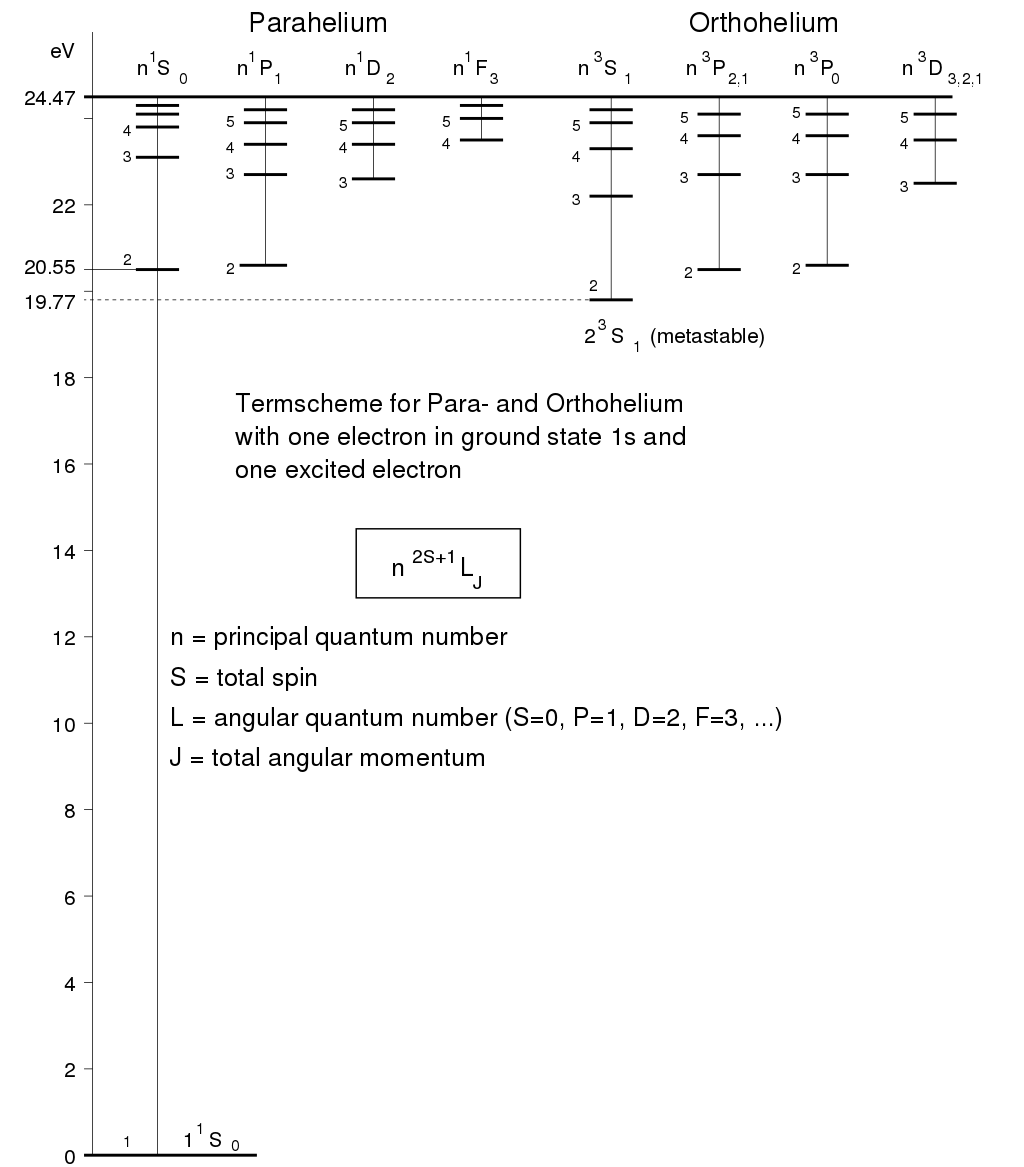
\includegraphics[width=5cm]{../Bilddateien/Helium-term-scheme.svg.png}
            \caption{Termschema des Heliumatoms aus \cite{wiki:helium-atom}.}
        \end{figure}
        Es gibt zwei Zustände des Wasserstoffatoms, einmal den Singulettzustand $1^1S_0$ und den Triplettzustand $1^3S_1$. 

        Für den Hamiltonoperator des Heliumatoms gilt der Zusammenhang
        \[
            H_\textit{He} = \bbbra{\ubra{\frac{P_1^2(x_1)}{2m_e} + \frac{P_2^2(x_2)}{2m_e} - \frac{2\cdot e^2}{4\pi\epsilon_0\cdot\dabs{x_1}{}} - \frac{2\cdot e^2}{4\pi\epsilon_0\cdot\dabs{x_2}{}}}{=:H_{\textit{He},0}} + \ubra{\frac{e^2}{4\pi\epsilon_0\cdot\dabs{x_1-x_2}{}}}{H_{e-e}}}_{x\in(\R^3)^2}.
        \]
        Die Wellenfunktion hat dann die Form 
        \[
            \Psi(x_1,x_2) = \psi_{1,0}(x_1,x_2)\cdot\chi_{1,0}(s_1,s_2)\cdot\chi_{0,0}(m_{s_1},m_{s_2}),
        \]
        wobei $\psi_{1,0}$ die Wellenfunktion des Wasserstoffatoms ist. Die Spinwellenfunktion ist dabei gegeben durch
        \[
            \chi_{1,0} = \frac{1}{\sqrt{2}}\cdot\bbra{\ket{\uparrow\downarrow} - \ket{\downarrow\uparrow}}.
        \]
        Die Gesamtwellenfunktion ist dann antisymmetrisch, da die Spinwellenfunktion antisymmetrisch ist. Für das Eigenwertproblem ohne Elektron-Elektron Wechselwirkung der Form $H_{\textit{He},0}\Psi = \lambda\cdot\Psi$ erhalten wir dann eine Eigenwertfolgensumme $E_{\textit{He},0} = E_{x_1} + E_{x_2}$. Dabei ist $E_{\textit{He},0}$ gegeben durch $E_{\textit{He},0} = \bbra{-R_y\cdot 2\cdot Z^2/n^2}_{n\in\N}$, wobei $R_y = 13.6\cdot\text{eV}$ die \emph{Rydberg-Energie} ist. Dadurch ergibt sich für $E_{\textit{He},0}(1) = -8\cdot R_y \approx -108.8\cdot\si{\electronvolt}$. Diese Energie müssen wir jedoch noch durch die Elektron - Elektron Wechselwirkung korrigieren; diesen Korrekturterm erhalten wir durch
        \[
            E_{\textit{He},1} = \braopket{\psi}{H_{e-e}(x)}{\psi} = \frac{5}{4\cdot a_0}\cdot\bbbra{\frac{e^2}{4\cdot\pi\cdot\epsilon_0}} \approx 34\cdot\si{\electronvolt}.
        \]
        Damit erhalten wir die Summe $E_{\textit{He},0} + E_{\textit{He},1} \approx -108.8\cdot\si{\electronvolt} + 34\cdot\si{\electronvolt} \approx -74.8\cdot\si{\electronvolt}$.
        \begin{Aufgabe}
            \nr{} Recherchiere zu dem versteckten Integral des Skalarproduktes und dessen Lösung. 

            \nr{} Aus der Störtheorie wissen wir, daß nur kleine Störungen zu guten Ergebnissen führen. Warum ist dies hier nicht der Fall? Durch welche Methoden können die Ergebnisse verbessert werden?
        \end{Aufgabe}
        In einem angeregten Singulett bzw. Triplett Zustand ergeben die Energieterme der Elektron-Elektron Wechselwirkung in der Skalarproduktauswertung mit den Wellenfunktionen $\psi^\textit{sing}$ bzw. $\psi^\textit{trip}$ die Separierung
        \begin{align*}
            E_{e-e}^\textit{sing} &= \Braopket{\psi^\textit{sing}}{H_{e-e}}{\psi^\textit{sing}} = I + J, \\
            E_{e-e}^\textit{trip} &= \Braopket{\psi^\textit{trip}}{H_{e-e}}{\psi^\textit{trip}} = I - J.
        \end{align*} 
        Dabei sind $I$ und $J$ Abkürzungen für komplizierte mehrdimensionale Integralausdrücke. Dabei bedeutet $I$ die \emph{Coulomb-Wechselwirkung} und $J$ die \emph{Austausch-Wechselwirkung}. Es spiegelt die Energie wieder, welche zwischen den beiden Elektronen bei einem Übergang ausgetauscht wird.
        \begin{Aufgabe}
            \nr{} Recherchiere zu den Integralen $I$ und $J$ und notiere deren Ausdrücke, indem du die Namen beider anhand ihrer Integranden verifiziertst. Ziehe dazu die Seite zum \href{https://de.wikipedia.org/wiki/Austauschwechselwirkung}{Austauschintegral} herbei.
        \end{Aufgabe}


\end{document}